\chapter{Introduction}
\label{chap:intro}

\paragraph{The problem.} Identifying an object from any perspective is a fundamental capability for intelligent vision systems that operate with multiple cameras. \textit{Cross-view object correspondence} aims
at matching objects across complementary viewpoints and underpins a growing class of real-world applications. In human-robot collaboration, an aerial vehicle and a ground-based human operator must agree on which
object in the scene is being referenced, despite observing it from entirely different angles \cite{collab_1, collab_2}. Augmented reality assistants face the same requirement; a camera mounted on the head
captures the user's immediate environment, while a fixed camera provides broader context of the scene \cite{wearable}. The growing adoption of consumer smart glasses means that these capabilities can be extended
to everyday personal use, for instance an application that helps a user find an object in his/her home by relating what the glasses see with the feed of a house camera. Another application is multi-robot
manipulation, where independent agents with non-overlapping fields of view must coordinate around shared objects without access to a common reference frame \cite{multirobot_1, multirobot_2}. In each of these
domains, failure is costly, since a system that cannot identify the same object across views cannot collaborate, cannot respond to instructions, and cannot be deployed safely. Despite steady progress in object
segmentation on single images, cross-view segmentation in video remains largely an open challenge.

\paragraph{The dataset.} The most comprehensive public resource for studying this problem is the \textit{Ego-Exo4D} dataset \cite{grauman2024egoexo4d}. It holds thousands of video recordings of human activities
captured simultaneously from a first-person \textit{egocentric} camera worn by the participant and one or more \textit{exocentric} cameras fixed around the scene. The dataset enables many novel computer vision
tasks, including cross-view object correspondence: given a per-frame segmentation mask track for an object in one camera view, predict the mask track for the same object in the other view.
\cref{fig:ego-exo-example} shows qualitative examples for both correspondence directions. The task is particularly demanding because the two perspectives focus on different aspects of the same scene. On the one
hand, the egocentric view captures object detail and manual interactions with high fidelity, but suffers from motion blur, frequent hand occlusion, and a narrow field of view that misses scene context. On the
other hand, the exocentric view provides a global picture of the environment and the person's body, but sacrifices detailed resolution for each individual object. As a result, the same object across the two
views appears at drastically different scales, angles, positions in the frame, and even colour brightness due to differing lighting conditions. 

\newpage
\noindent Moreover, the cameras lack geometric calibration information, which
renders triangulation-based approaches unfeasible. Finally, the wide variety of recorded scenes, camera optics, and imaging conditions introduces a broad domain shift range that challenges any vision perception
method developed on a standard image dataset.

\begin{figure}
    \centering
    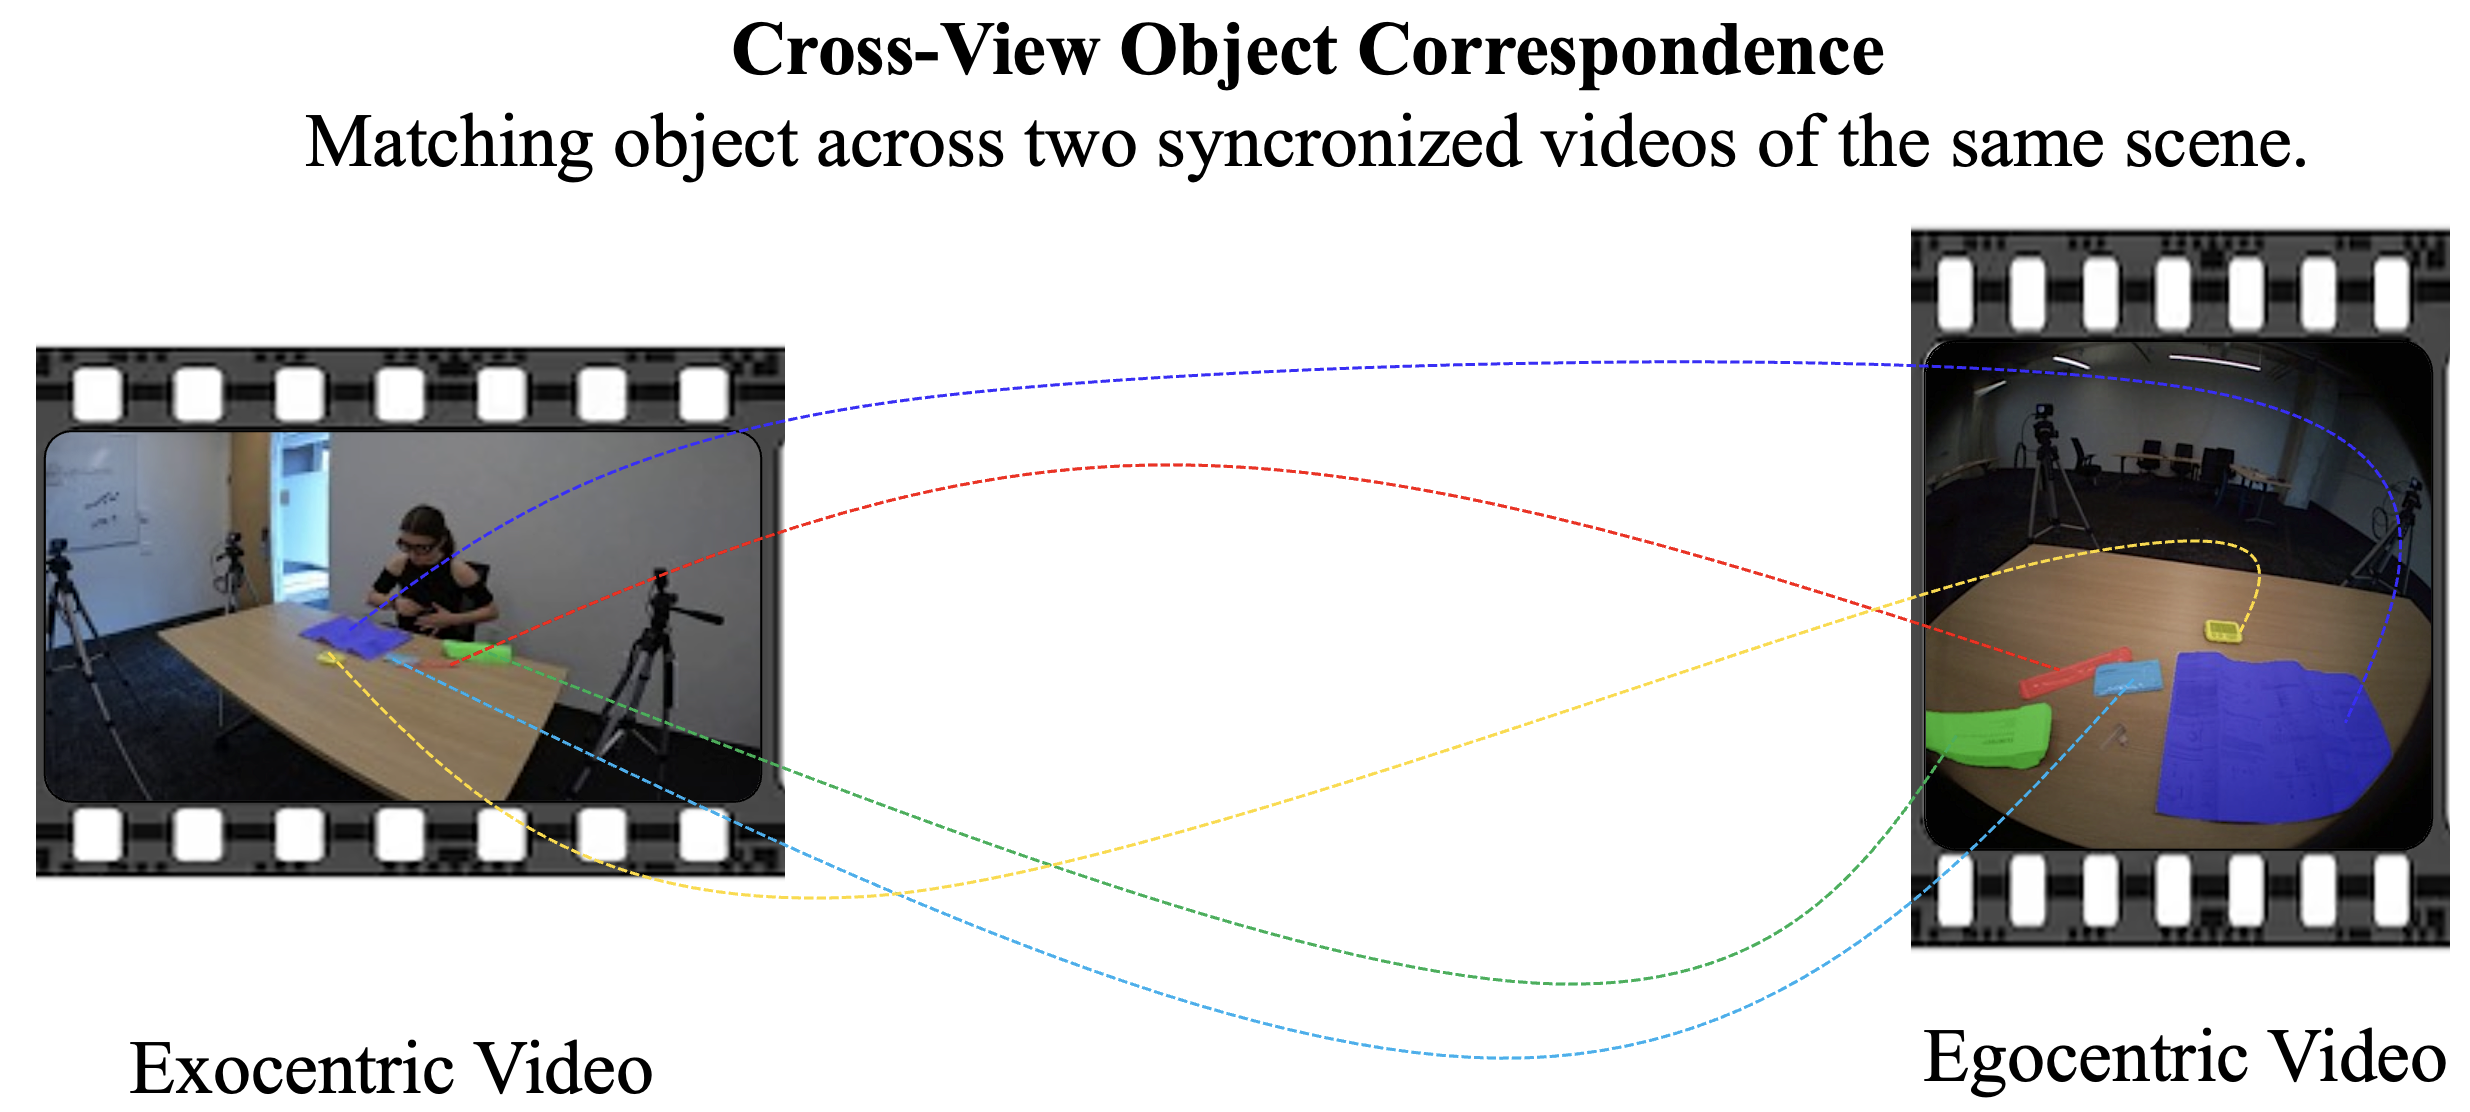
\includegraphics[width=0.8\linewidth]{latex/imgs/ch1/cross-view-intro.png}
    \caption{The Cross-View Object Correspondence Task.}
    \label{fig:placeholder}
\end{figure}

\begin{figure}
  \centering
  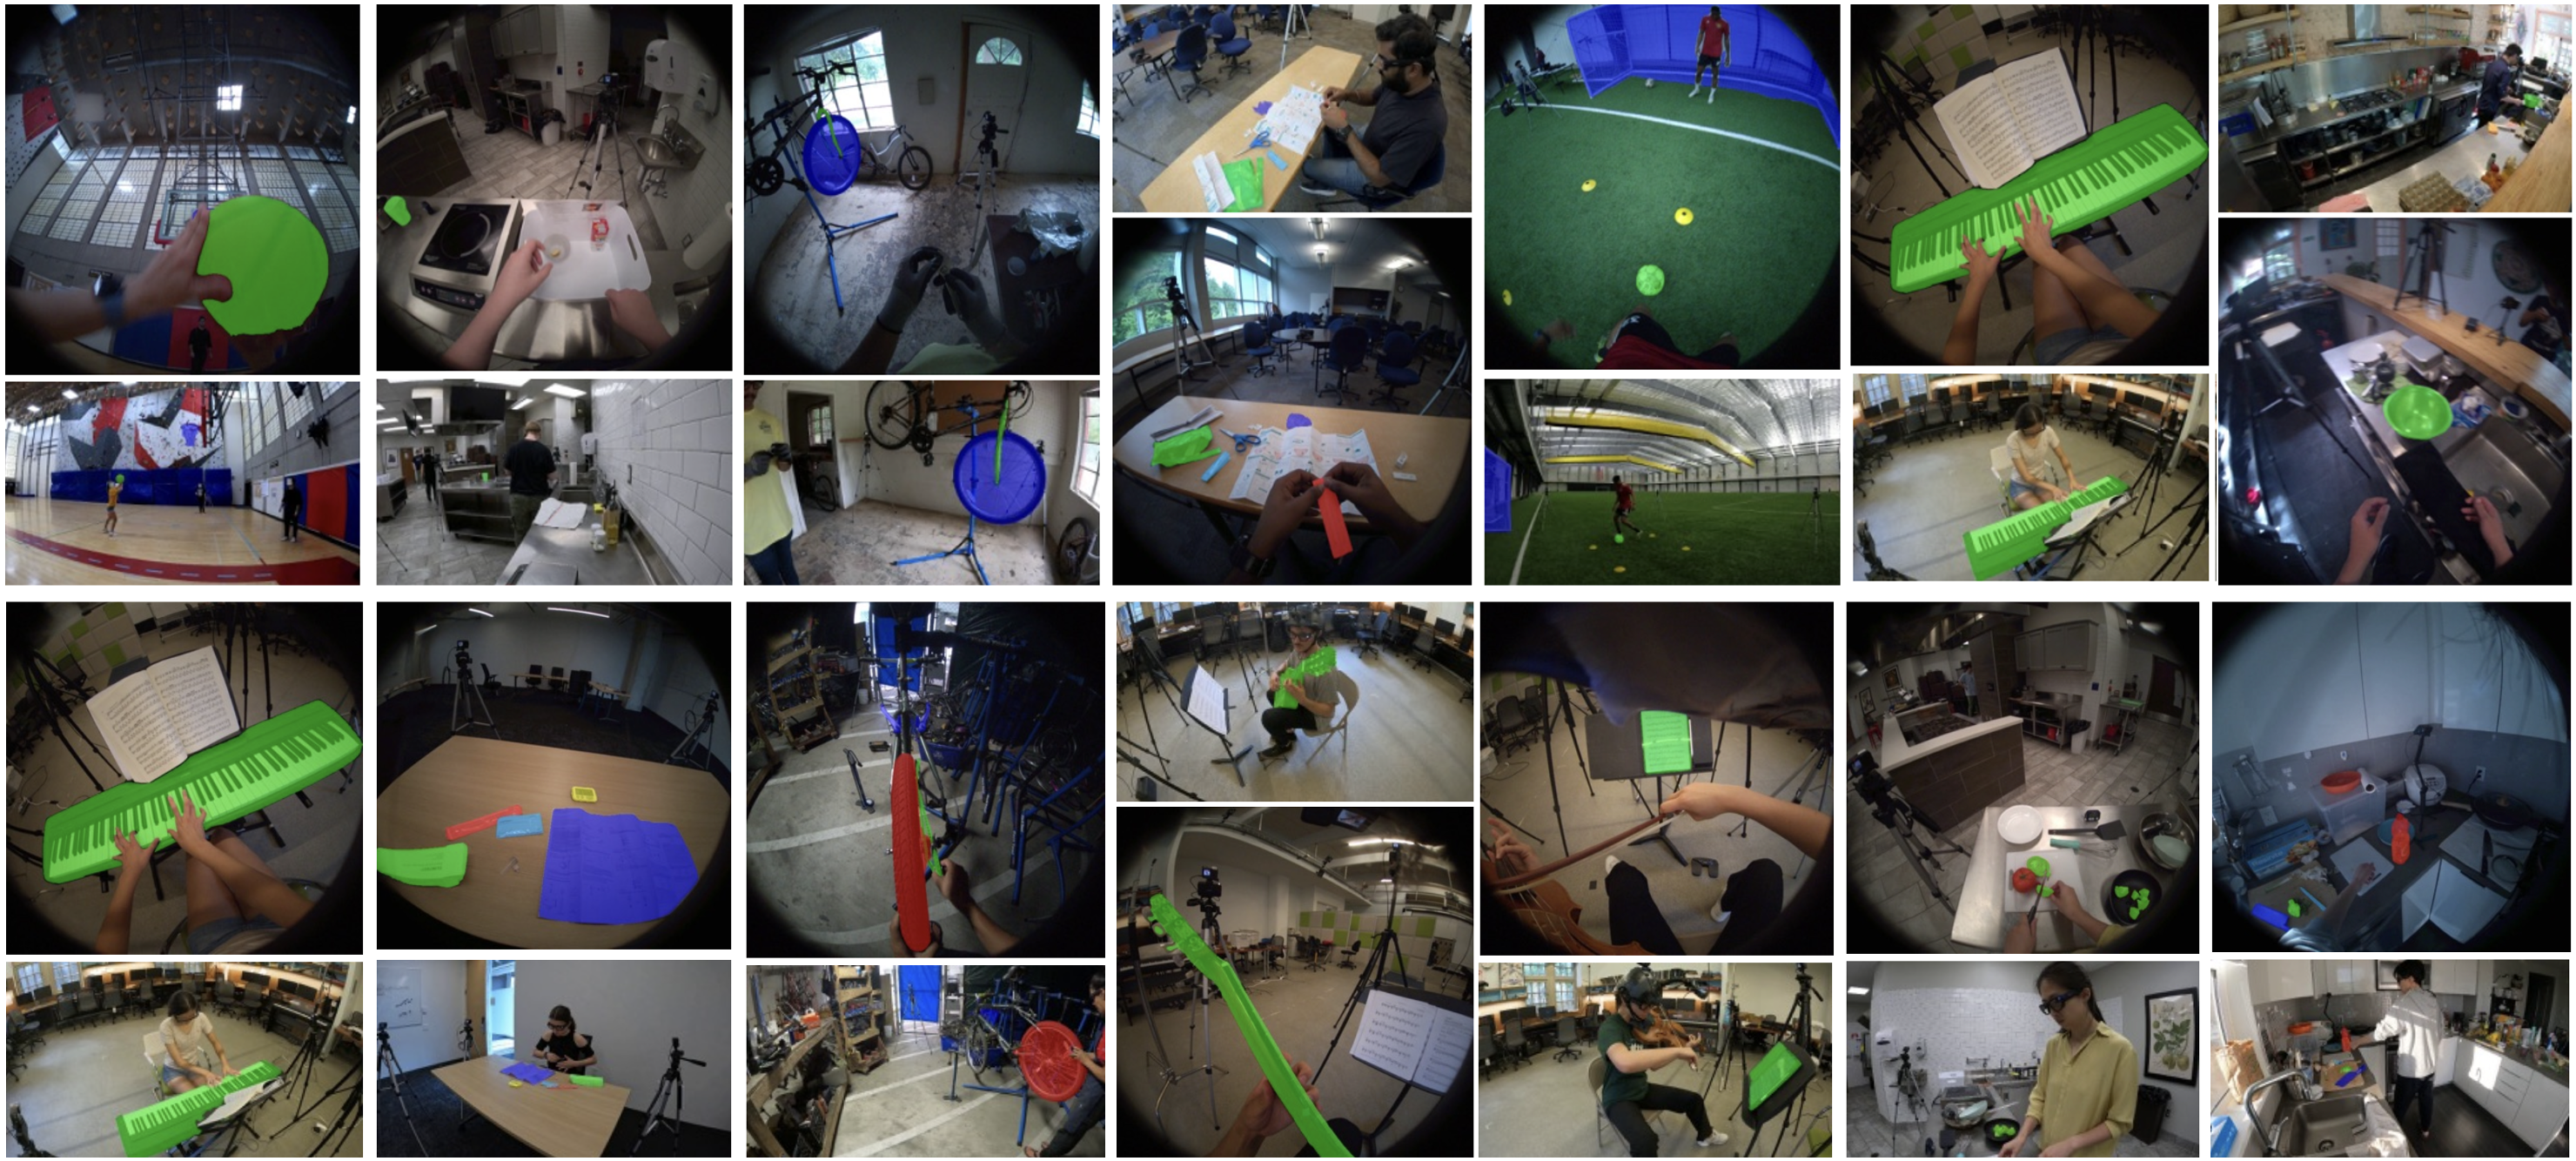
\includegraphics[width=1\linewidth]{latex/imgs/ch1/egoexo-many-examples.png}
  \caption{Qualitative examples of cross-view object correspondence. Couples of frames are displayed vertically. Different objects in the same frame are marked with mask overlays of different color.}
  \label{fig:ego-exo-example}
\end{figure}

\paragraph{Existing solutions.} Current state-of-the-art methods address this challenge by encoding objects into embeddings and then learning how to match them across views. To date, LM-EEC by Hu et al.\ (2025)
\cite{hu2025lmeec} achieves the strongest published results. It adapts SAM~2 with a Mixture-of-Experts fusion module and a dual compressed long-term memory system optimised for object segmentation on long
videos.  O-MaMa \cite{o-mama}, the winner of the 2025 Ego-Exo4D Correspondences Challenge \cite{leaderboard}, generates candidate
masks in the destination view via FastSAM and selects the best match using pooled DINOv2 features in a learned cross-view latent space. \cite{pan2025v2sam} take a complementary route, adapting SAM~2 with dual
prompt generators and a cyclic-consistency selector. All related works will be explored in depth in \cref{chap:theory}. While they achieve respectable results, all these approaches share two crucial limitations.
First, they rely on training pipelines, which ties each model to the distribution of available Ego-Exo4D training data, making them inapplicable to novel camera configurations or scenarios without retraining.
Second, the predictions they produce are difficult to interpret, since the rationale behind any segmentation is ingrained between model weights, architecture components, and abstract vector embeddings with
hundreds of entries; only attention maps can be used to inspect why a particular object was segmented in a particular frame. This hinders their applicability in the real world, where accountability requires that
every decision be explainable and where the owners of computer vision systems must answer for the outcomes those systems produce \cite{xai-sensors}.

\paragraph{Foundation models.} Over the last five years, a new paradigm in machine learning emerged: foundation models. The emergence of large language models has demonstrated across a wide range of settings
that systems trained on broad data and used without task-specific fine-tuning can match or exceed specialists \cite{wu2023exploringtradeoffsunifiedlarge, kim2023languagemodelssolvecomputer,
gruver2024largelanguagemodelszeroshot}. A similar transition is happening in computer vision. Currently, most problems are addressed by designing task-specific architectures and collecting task-specific
supervised data. In contrast, LeCun and others
\cite{maes2026leworldmodelstableendtoendjointembedding, assran2025vjepa2selfsupervisedvideo, dinov1}
argue that self-supervised learning on video data is the most promising path towards building models that understand world dynamics at a truly foundational level. While text is already an abstract compression of
information, video data inherently captures information about physics, object permanence, causality, and the consequences of action. Therefore, if a model has internalised how the world works, it develops the
kind of competence that should transfer across tasks and modalities. Our work is inspired by this philosophy: if foundation models with vision capabilities have acquired a sufficiently general understanding of
the visual world, carefully composing them at inference
time should transfer to novel tasks that none was designed for.

\paragraph{Language as a bridge hypothesis.} Following the above observations on the limits of current methods, and the emergence of general-purpose foundation models, we ask ourselves: can natural language
serve as a bridge between machine learning architectures, acting as a simple yet effective medium for compressing information that replaces complex learned features? The question is relevant for two reasons.
First, it mirrors how humans collaborate.  Each of us perceives a scene, describes it in language, and sends a message to others who rely on language to coordinate and achieve a common goal. Crucially, natural
language is the most effective tool for us. While mathematics would be more precise and efficient at compressing information, it is expensive to generate and not accessible to everyone. Second, a system built on
natural language is interpretable by design. A pipeline whose modules communicate through a natural text exposes every step of the reasoning process, so that any prediction can be inspected, and any unsafe or
erroneous output can be verified and stopped. 

\newpage
\noindent Cross-view object correspondence on \textit{Ego-Exo4D} provides a concrete testing ground to this question since it directly simulates two agents with different
perspectives who use language to coordinate actions and find a common physical object.
\begin{figure}[H]
  \centering
  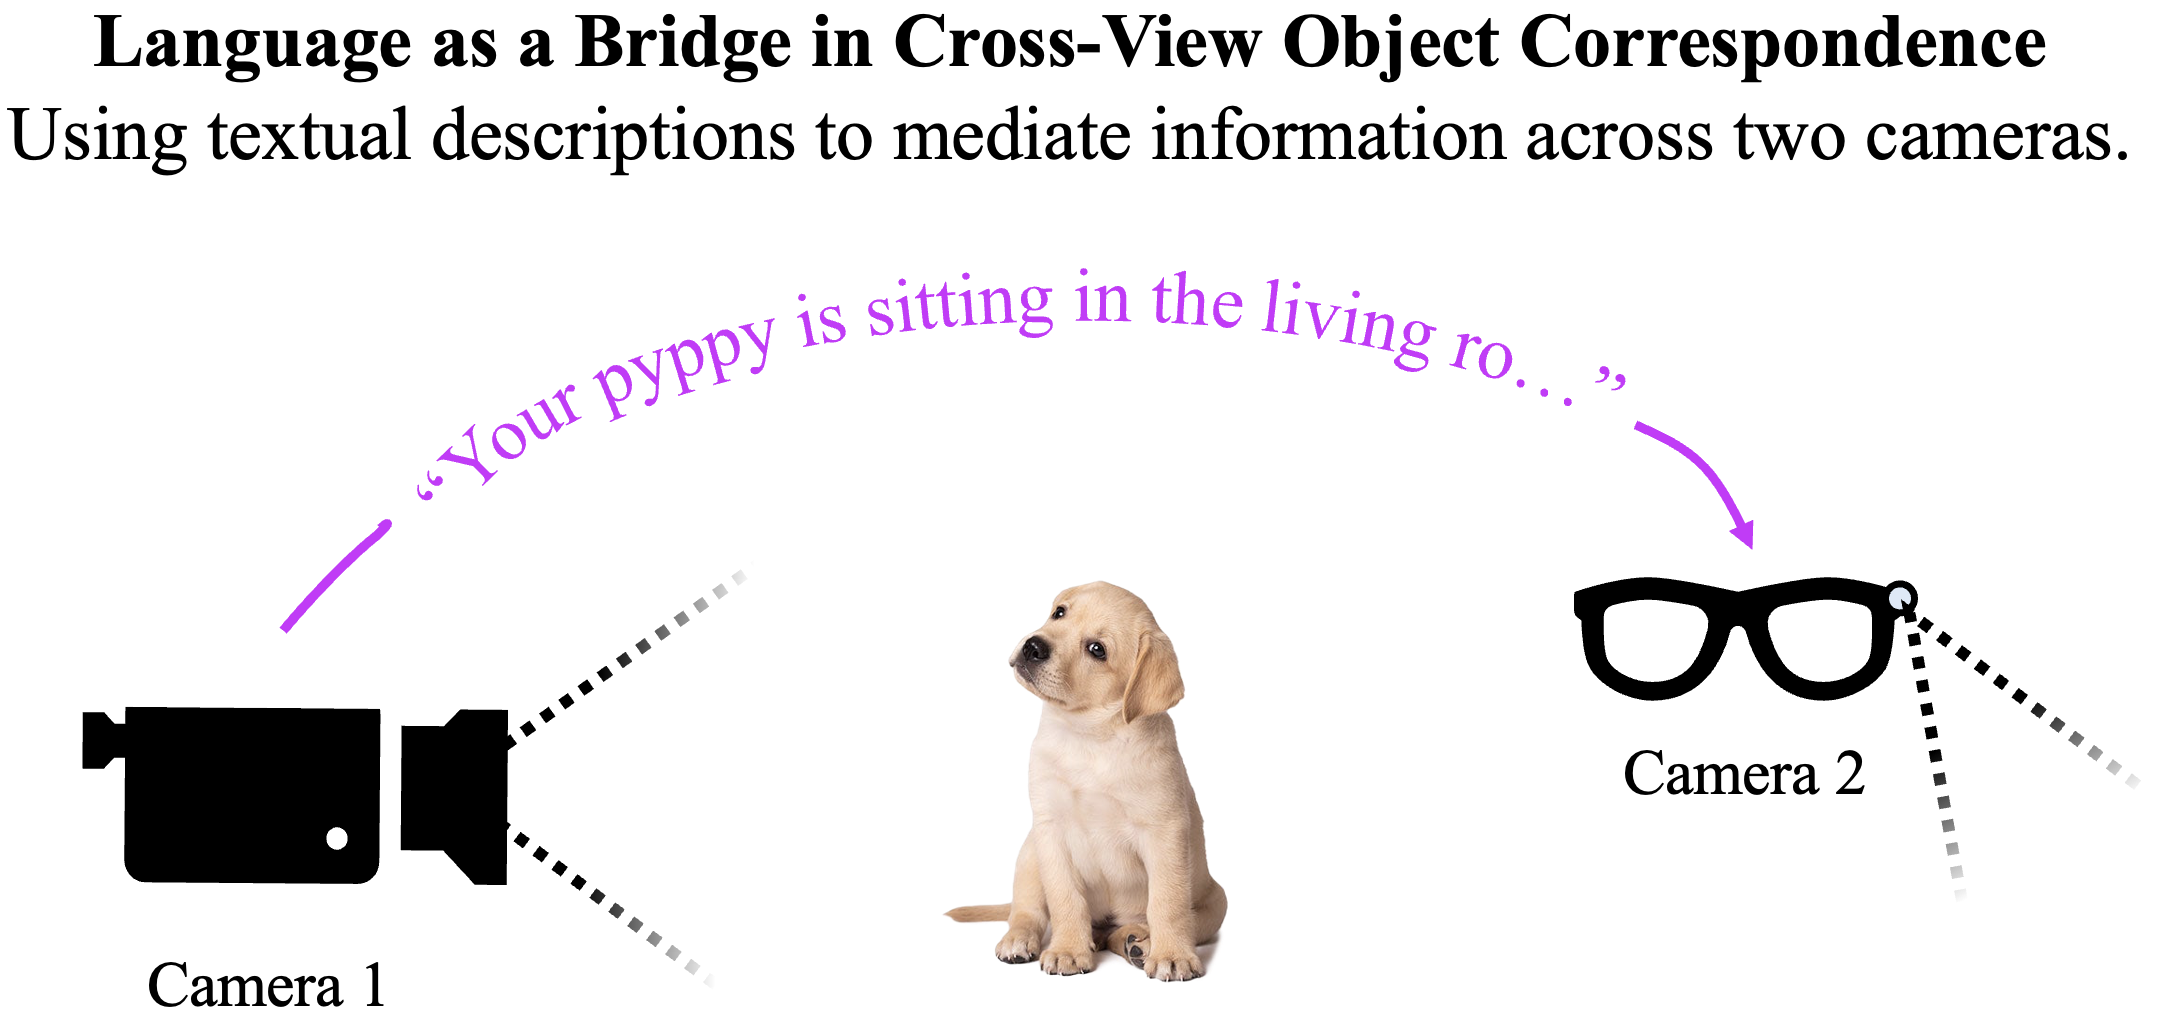
\includegraphics[width=0.8\linewidth]{latex/imgs/ch1/lang-bridge-intro.png}
  \caption{Illustrative example of language acting as a bridge in a system of two cameras that helps its user to find objects (and animals) in its house.}
  \label{fig:pipeline-summary}
\end{figure}

\paragraph{Our Pipeline.} To this end, we propose the ``two eyes and one mouth'' pipeline. Two cameras observe the scene from complementary perspectives, and a single natural language description mediates the
object correspondence between them, illustrated in \cref{fig:ego-exo-example}. Given a source-view mask track, we first select the single highest-quality seed frame from the source view and pass it to a visual
large language model, which generates a view- and time-independent description of the target object. That description then drives two coordinated processes. First, an open-vocabulary detector scores destination
frames by object-text alignment to select the most informative anchor frames. Second, a SAM~3 agentic loop localises and segments the object in each anchor frame using the same description as the grounding
signal. Finally, SAM~2's video tracker completes the mask track across all remaining destination frames by propagating predictions conditioned on a memory bank of anchor and recently processed frames.

Crucially, no component of the pipeline is fine-tuned for the task. Because it inherits no dependence on the distribution of any cross-view dataset, the pipeline is in principle both camera and dataset agnostic,
meaning that it can be applied to novel camera configurations and scenarios without retraining, directly addressing the first limitation of existing solutions.
The bridge between views is a human-readable JSON description, and any erroneous prediction can be localised to the specific block whose output is at fault.

Our pipeline achieves $37.7$ (\textit{Ego2Exo}) and $40.6$ (\textit{Exo2Ego}) IoU on the \textit{Ego-Exo4D} Correspondences v2 test split, representing a relative gain of $9\%$ and $62\%$ against the official
challenge baselines respectively. These results place our approach within a few percentage points of O-MaMa \cite{o-mama}, the 2025 challenge winner, all without any training on cross-view data.

\paragraph{Thesis overview.} We begin this dissertation in \cref{chap:theory} by establishing the theoretical foundations that underpin our pipeline, covering transformers, visual representation, self-supervised
learning, promptable segmentation in video with the Segment Anything family, open-vocabulary language grounding, large language and vision models, and how to design an LLM agent. We conclude the review with a
recap of the related methods for cross-view object correspondence, exploring their architectures. In doing so, we highlight the common limitation, which sets us up for the main contributions of the thesis. In
\cref{chap:pipeline}, we describe the full pipeline, motivating each design choice with the explored theoretical concepts. In \cref{chap:experiments}, we present the results, further motivate the construction of
our pipeline with an ablation study, and discuss its performance. We outline the advantages but deliberately focus on the failure modes to study how the chosen foundation models behave on a task none of them
was designed for. \cref{chap:conclusions} wraps our findings together and proposes research directions for the future. Together, this work demonstrates that a composition of general-purpose foundation models mediated by language constitutes a viable, interpretable, and training-free alternative for cross-view
object correspondence, a task previously dominated by specialised learned architectures, which in turn suggests that natural language can be a reliable bridge among machine learning architectures and opens this
novel paradigm for future research.